\cleardoublepage

\chapter{Descripción del sistema}
\label{makereference2}

\section{Introducción}
\label{makereference2.1} 
% Aquí hay que introducir algo, pero maaaajo ni idea

\section{Nodo}
\label{makereference2.2}

El nodo cuenta con una Raspberry Pi modelo 2b con Raspbian a la que están conectados dos sensores: DHT22 (temperatura y humedad) y un piranómetro~\ref{figure2}.
Gracias a la ayuda de los 'datasheets' proporcionados por los fabricantes de los dispositivos, comprendimos cómo era el funcionamiento de estos. 
Las llamadas al sensor se realizan a través de su API en Python, proporcionada por Adafruit, lo cual nos facilitó mucho el trabajo de recolección de datos.

En el nodo corre un script que se encarga de recoger los datos del exterior y enviarlos vía MQTT al servidor para, más adelante, ser procesados.

\section{Servidor}
\label{makereference2.3}

El servidor es una máquina física alojada en la Facultad de Físicas de la Universidad Complutense de Madrid. Nos proporcionaron un usuario y una contraseña para poder acceder por SSH y trabajar en remoto. Necesitamos una máquina de este calibre debido a la gran cantidad de datos a ser tratados y, sobre todo, al proceso de entrenamiento de estos.

Aquí, guardaremos o descargaremos los ficheros CSV que vamos a utilizar para las pruebas y entrenamiento final. De esta manera, nos ha servido para estudiar los distintos algoritmos de 'machine learning' y ver cuál de ellos se ajusta mejor a nuestro proyecto.

Con el algoritmo elegido, hemos lanzado el entrenamiento final. Así, el servidor estaría preparado para predecir la radiación a partir de los datos recibidos del nodo.

Cuando la máquina obtiene una predicción, esta será enviada a ThinkSpeak, donde será representada.

\section{ThingSpeak}
\label{makereference2.4}

ThinkSpeak es una aplicación de código abierto que permite llevar un registro de los datos que se desean. Permite representarlos y estudiarlos.

En nuestro caso, el servidor enviará la predicción junto a la hora a la que debería ocurrir. ThinkSpeak se encarga de representar estos datos en una gráfica junto a la radicación real en esa hora, para poder ver el error respecto a la realidad.

\begin{figure}[htb]
	
	\begin{center}
		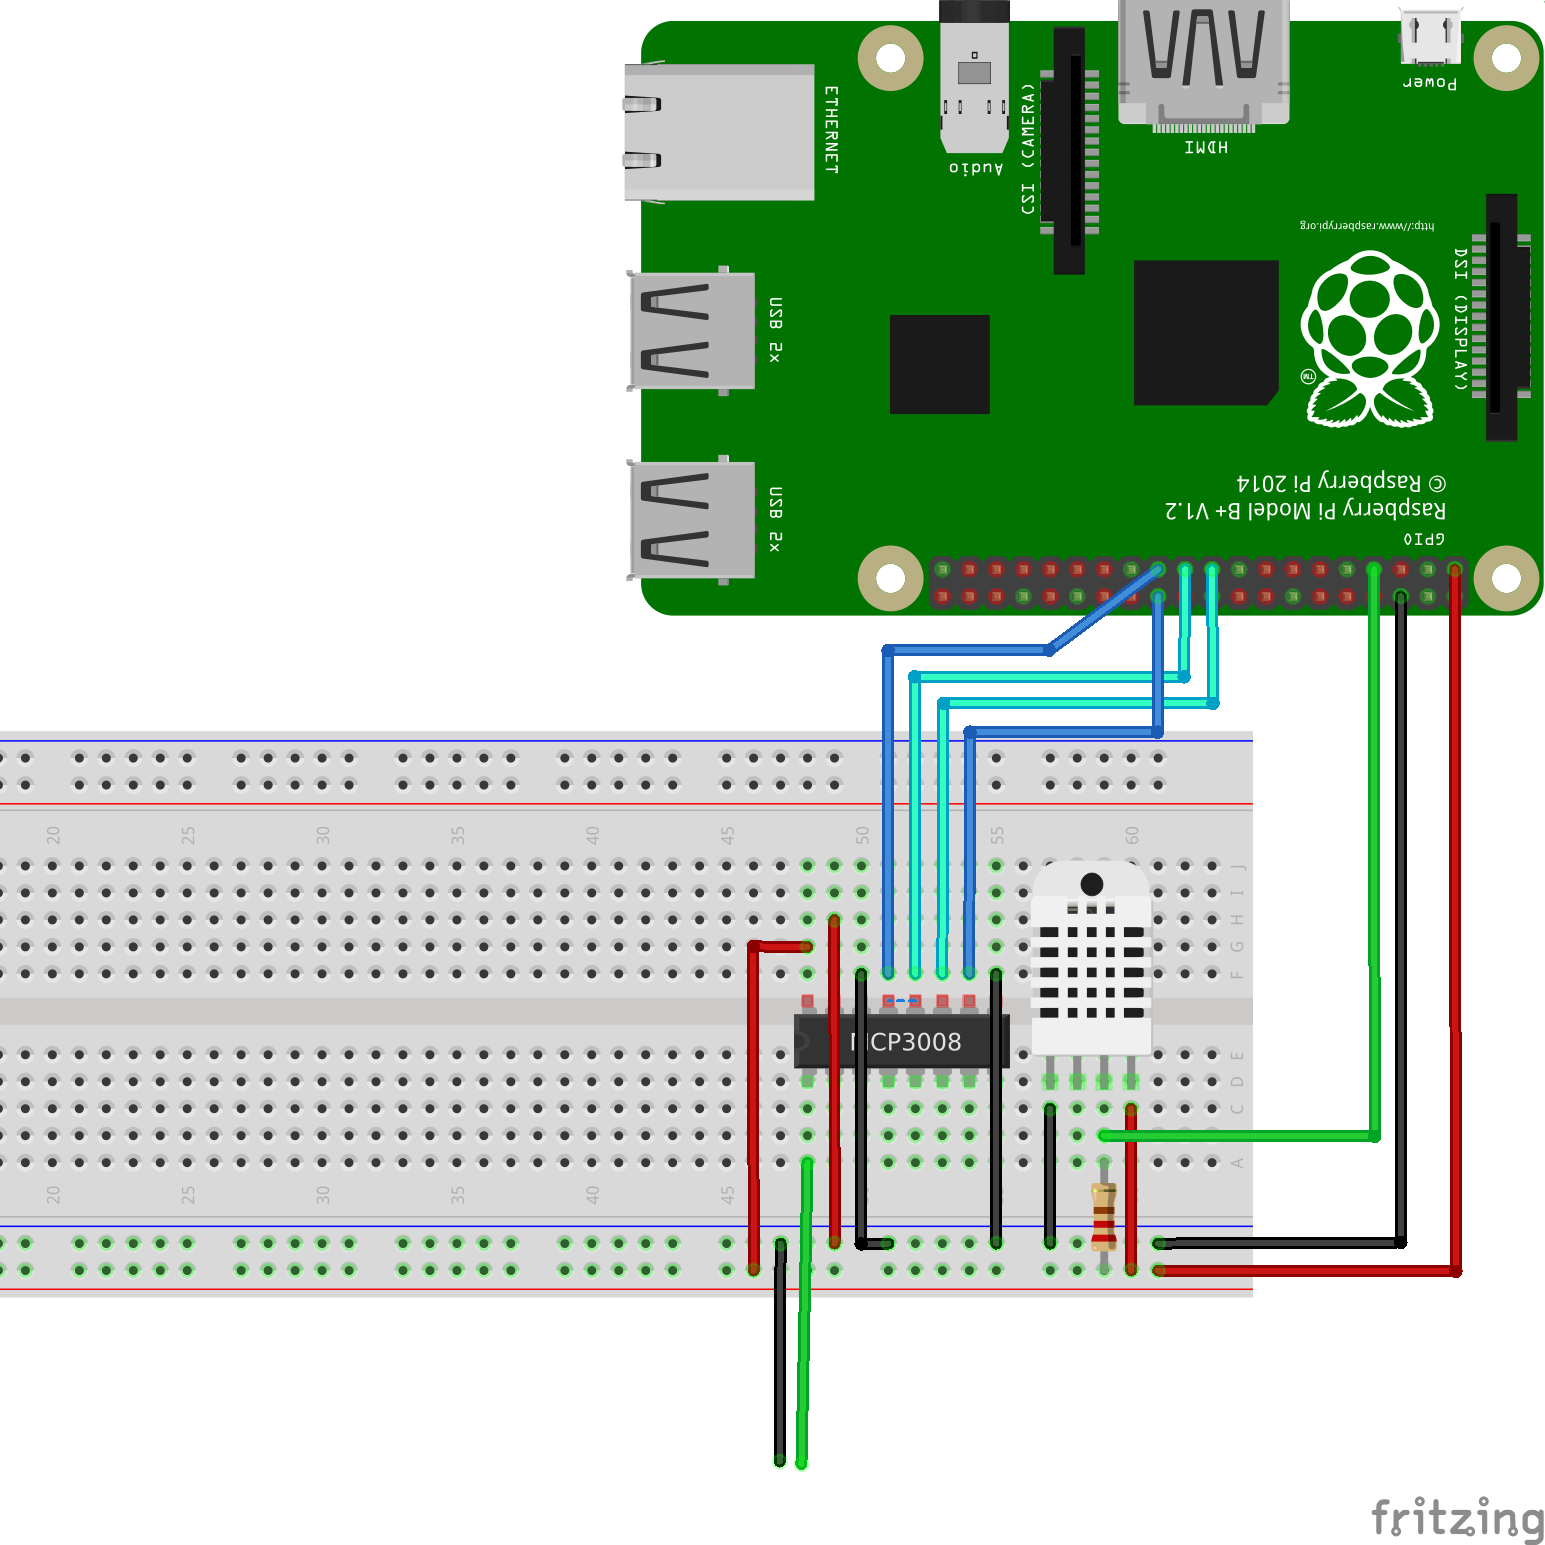
\includegraphics[width=15cm,height=15cm]{figures/solar_project_node_diagram.png}
		\caption{Diagrama del nodo}
	\end{center}
	
	\label{figure2}
\end{figure}